%%%%%%%%%%%%%%%%%%%%%%%%%%%%%%%%%%%%%%%%%%
\section{Heat Transport in Packed Beds} \label{sec:modeling-heat-transfer}
%%%%%%%%%%%%%%%%%%%%%%%%%%%%%%%%%%%%%%%%%%
In our analysis of the momentum of packed beds, we focused entirely on the exchange of momentum between a fluid passing through a packed bed. The mechanics of contacting particles will be dealt with entirely within the framework of the discrete element method, to be discussed in \cref{sec:modeling-dem}. But now as we move to analyze the heat transfer in a packed bed, we will consider both inter-particle modes of heat transfer as well as particle-fluid convection. 


\begin{figure}[t]
	\centering
	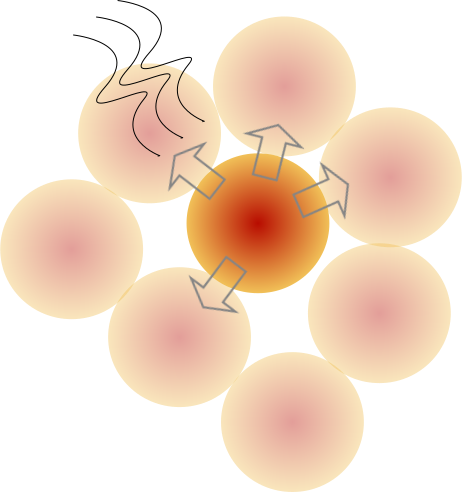
\includegraphics[width=0.35\textwidth]{chapters/figures/pebble-complete-heat-transfer}
	\caption{An illustration highlighting a single particle transferring energy into a passing fluid and neighboring particles in the ensemble.}\label{fig:peb-comp-ht}
\end{figure}

Looking at the particle highlighted in Fig.~\ref{fig:peb-comp-ht}, we see many pathways for heat to be transferred inside the ensemble. The most significant are:

\begin{enumerate}
\item Conduction through the contact area between contacting particles.
\item Conduction through the stagnant fluid between near, non-contacting particles.
\item Conduction through the stagnant fluid between contacting particles.
\item Advection of energy by the fluid to contacting- and downstream particles.
\item Radiation between the surfaces of contacting particles.
\item Radiation between particles of adjacent voids.
\item Heat generation internally in the particle.
\end{enumerate}

We will address the inter-particle conduction in \cref{sec:ht-pebble-conduction} wherein we derive a formula for heat conductance between contacting, elastic spheres. The complex interaction of energy in a particle with a fluid (conduction through film regions, convection with passing fluid, etc.) will all be dealt with using correlations for packed beds; this is done in \cref{sec:particle-convection}. We will briefly discuss some literature where researchers have dealt with the radiation between particles in a packed bed but do not include the terms in our current models. Finally, the last mode of heat transfer is trivially accounted for with a heat source term,

\begin{equation}\label{eq:nuclear-heating-term}
	Q_g = q'''V
\end{equation}

where $q'''$ is a known volumetric heating rate and $V$ is the volume of our particle. In practice, we will know a volumetric heating rate from the location and geometry of the solid breeder volume. The volume of the sphere is $V = \frac{\pi}{6} d_p^3$.

In the following sections we will expand upon the details of the modes of heat transfer considered for our packed beds. They forms of equations used will be written in a way as to be easily implemented directly into the DEM computational framework, to be discussed later in \cref{sec:modeling-dem}.

% The transient energy balance for an irradiated pebble, shown in Fig.~\ref{fig:peb-comp-ht}, in a packed bed with flowing interstitial gas is given by Eq.~\ref{eq:single-pebble-energy},

% \begin{equation}\label{eq:single-pebble-energy}
% 	\rho V C \frac{\mathrm{d}T}{\mathrm{d}t} = \dot{Q}_g + \dot{Q}_\text{conduction} + \dot{Q}_\text{convection} + \dot{Q}_\text{radiation}
% \end{equation}



%%%%%%%%%%%%%%%%%%%%%%%%%%%%%%%%%%%%%%%%%%
\section{Inter-particle heat conduction}\label{sec:ht-pebble-conduction}

Handling the heat transfer between contacting particles has been investigated extensively by researchers in a number of fields\cite{Zhou2009,Zhang2011,Wu2011,Vargas2001,Li2000,Chaudhuri2006}.

In the Hertz analysis we walked through in \S\ref{sec:hertz-contact}, we found the contact radius of two elastic spheres in Eq.~\ref{eq:hertz-radius} as a function of the contact pressure. We rewrite the radius in terms of the compression force acting on the bodies,

\begin{equation}
	a =  \left(\frac{3}{4}\frac{R^*}{E^*}\right)^{1/3}F^{1/3}	
\end{equation}

where $\frac{1}{E^*} = \frac{1-\nu_1^2}{E_1} + \frac{1-\nu_2^2}{E_2}$ and $\frac{1}{R^*} = \frac{1}{R_1} + \frac{1}{R_2}$ as before.

Batchelor and O'Brien\cite{Batchelor1977} made the brilliant observation that the temperature fields in the near-region of contacting spheres are analogous to the velocity potential of the potential flow of a fluid passing from from one reservoir to another through a circular hole in a planar wall. With the analogy, they could make use of the fluid flow solution to write the total flux across the circle of contact,

\begin{equation}\label{eq:pebble-conduction-heat-transfer}
	Q_{ij} = H_{ij}(T_i - T_j)
\end{equation}

with the heat conductance, 

\begin{equation}\label{eq:batchelor-pebble-conductance}
	H_{ij} = 2k_sa = 2k_s \left(\frac{3}{4}\frac{R^*}{E^*}\right)^{1/3}F^{1/3}
\end{equation}

governing the time rate of energy transferred per temperature difference between particles, $T_i$ and $T_j$, respectively. This approach, laid out by Batchelor and O'Brien, is valid when the thermal conductivity ratio of solid and fluid is well above unity and the contact area is small relative to the particle. The condition is expressed as,

\begin{equation}
	\frac{ k_s }{ k_f } \frac{a}{R^*} = \lambda \gg 1
\end{equation}

The model, being derived from Hertz theory, also carries with it many of the assumptions and limitations inherent with that theory. The assumptions are discussed in detail in \S\ref{sec:hertz-contact}.

Recently, Cheng, et al.\cite{Cheng19994199} proposed a slightly modified variant of the conductance given by Batchelor and O'Brien. In their model, they allow for contacting materials of different thermal conductivity. Therefore they have,

\begin{equation}
	H_{ij} = 2k^*a = 2k^* \left(\frac{3}{4}\frac{R^*}{E^*}\right)^{1/3}F^{1/3}
\end{equation}

where $\frac{1}{k^*} = \frac{1}{k_i} + \frac{1}{k_j}$. As well as being a more general, flexible formulation, the models analyzed by Cheng, et al.\cite{Cheng19994199} are in good agreement with experiments and will be used in this study.






\subsubsection{Large Biot number}
Considering now material and geometric properties relevant to our ceramic pebble beds, we will see that we may need to consider the effects of a larger $\Bi$ for our pebbles. The helium purge gas moving through the packed beds is not specifically intended to act as a heat transfer agent and moves along at a creeping flow rate. For a first approximation we will therefore assume as a lower limit the Nusselt number is $\Nu = 2$ (the value for a sphere in quiescent fluid). From the requirement that $\Bi \ll 1$, we have

\begin{equation}
	2 \frac{k_f}{k_s} \ll 1
\end{equation}

The conductivity of helium over the temperature range of 300 to 800 $^\circ$C is approximately 0.3 \si{W/m-K}. The solid conductivity of \lit and \lis are approximately 2 \si{W/m-K}. Because of the low conductivity of our solid, the Biot assumption is barely valid, $0.3 < 1$. 

\section{Nusselt number for spheres in packed beds}\label{sec:particle-convection}

\subsection{Radiative transfer with neighboring particles}

The temperatures expected in the solid breeder are high enough that we can not a priori neglect radiation. The radiation exchange between contacting neighbors in a packed bed becomes extremely complex due to the local and semi-local nature of radiation. A standard approach to treat radiation exchange between surfaces is to consider the view factor between them. In a dense, randomly packed bed of spheres the computation of view factors between pebbles can be done via a method such as that proposed Feng and Han\cite{Feng2012}. Ideally, we could show this mode of heat transport is negligible compared to the others already discussed.

In ceramic breeder designs, the tritium breeding volume is rarely more than \si{2 cm} wide with pebbles that are, generally, \si{1 mm} in diameter. The maximum expected temperature in the breeding zone is about \si{1000 K}, roughly at the centerline of the \si{2 cm} width. The walls of the coolant must be held below the operable steel temperature of roughly \si{700 K}. This works out to a \si{300 K} differences spanning 10 pebble diameters. From this we can make a first-order approximation of \si{30 K} difference between neighboring pebbles. At the elevated temperatures, an estimate for the radiation exchange between two pebbles (allowing them to act as black bodies for this approximation) is

\begin{equation}
	\dot{Q}_\text{radiation} = \sigma A \left(T_\text{max}^4 - (T_\text{max}-30)^4\right) \approx 0.022\si{W}
\end{equation}
 
 which is the highest amount of radiation exchange we might expect between pebbles. Even though we will neglect this mode of heat transfer for now, after reviewing some of the packed bed heat transfer results we may find that this quantity of energy transfer is not negligible and future versions of the model would have to account for it.
%%%%%%%%%%%%%%%%%%%%%%%%%%%%%%%%%%%%%%%%%%
